\documentclass[tikz,border=12pt]{standalone}
\usepackage[T1]{fontenc}
\usepackage{mathpazo}
\usepackage{amsmath,amssymb}
\usetikzlibrary{arrows.meta, positioning, calc, fit, decorations.pathreplacing}

\definecolor{stblue}{HTML}{7B97AD}
\definecolor{rwgold}{HTML}{B8995E}
\definecolor{sage}{HTML}{7A9A7E}
\definecolor{dkbrown}{HTML}{3D3530}
\definecolor{wmgray}{HTML}{7B7067}
\definecolor{cream}{HTML}{F9F6F0}
\definecolor{border}{HTML}{D4C9B8}
\definecolor{terracotta}{HTML}{C47A6A}
\definecolor{lavender}{HTML}{907EA0}

\begin{document}
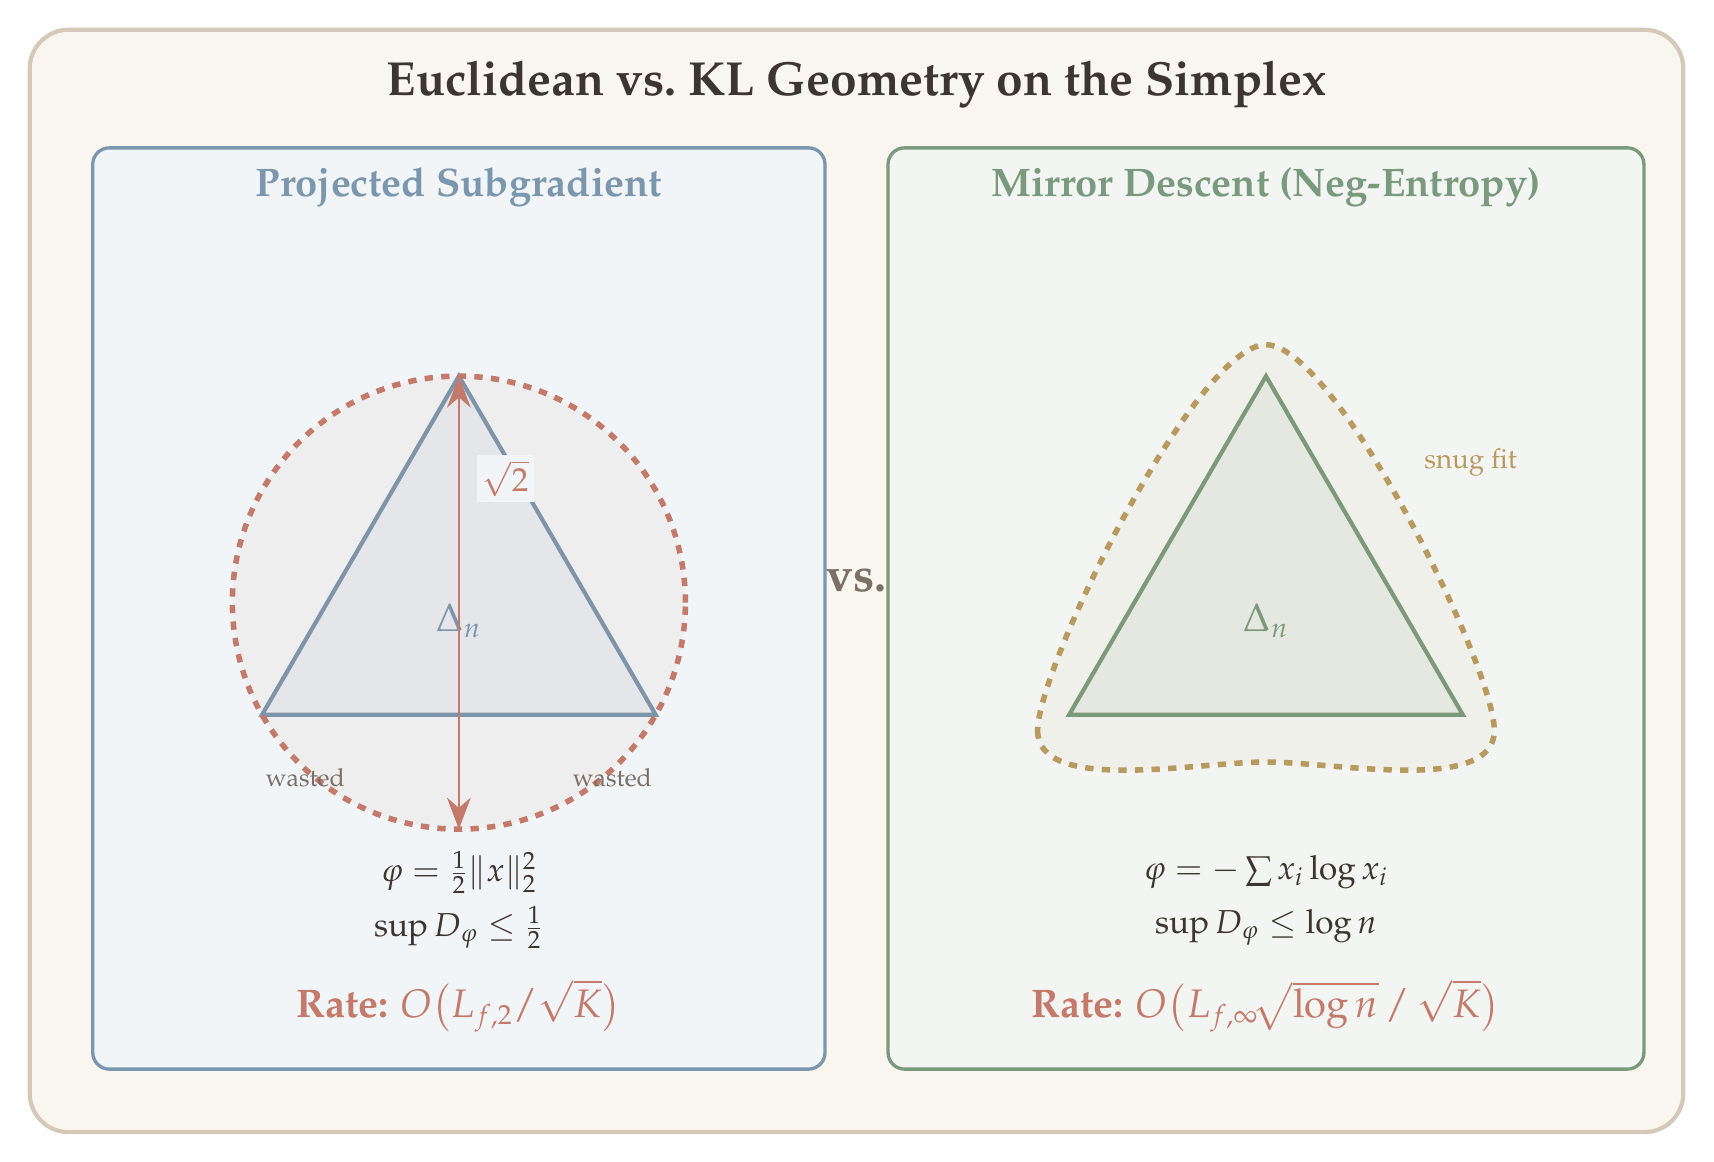
\begin{tikzpicture}[>={Stealth[length=4mm, width=3mm]}]

% Background
\fill[cream, rounded corners=14pt] (-0.5,-0.5) rectangle (20.5,13.5);
\draw[border, line width=1.5pt, rounded corners=14pt] (-0.5,-0.5) rectangle (20.5,13.5);

% Title
\node[text=dkbrown, font=\LARGE\bfseries] at (10,12.8) {Euclidean vs.\ KL Geometry on the Simplex};

% === LEFT: Euclidean ===
\fill[stblue!10, rounded corners=6pt] (0.3,0.3) rectangle (9.6,12.0);
\draw[stblue, line width=1.2pt, rounded corners=6pt] (0.3,0.3) rectangle (9.6,12.0);
\node[text=stblue, font=\Large\bfseries] at (4.95,11.5) {Projected Subgradient};

% Simplex triangle — smaller, centered at (4.95, 6.5)
% Equilateral-ish: base 5.0, height 4.3
\coordinate (LA) at (2.45,4.8);
\coordinate (LB) at (7.45,4.8);
\coordinate (LC) at (4.95,9.1);

\fill[stblue!18] (LA) -- (LB) -- (LC) -- cycle;
\draw[stblue, line width=1.5pt] (LA) -- (LB) -- (LC) -- cycle;
\node[text=stblue, font=\Large] at (4.95,6.0) {$\Delta_n$};

% Circumscribing circle
% Vertices: (2.45,4.8), (7.45,4.8), (4.95,9.1)
% By symmetry, circumcenter is at x=4.95
% Midpoint of LA-LC: (3.7, 6.95), slope LA-LC = 4.3/2.5 = 1.72, perp slope = -0.581
% Line: y - 6.95 = -0.581*(x - 3.7), at x=4.95: y = 6.95 - 0.581*1.25 = 6.224
% R = dist to (4.95, 9.1) = |9.1 - 6.224| = 2.876
% Check to (2.45, 4.8): sqrt(6.25 + 2.027) = sqrt(8.277) = 2.877 ✓
\draw[terracotta, line width=2pt, dashed] (4.95,6.224) circle (2.877);
\fill[terracotta, opacity=0.05] (4.95,6.224) circle (2.877);

% Diameter line
\draw[terracotta, line width=1pt, <->] (4.95,{6.224-2.877}) -- (4.95,{6.224+2.877});
\node[text=terracotta, font=\large, fill=stblue!10, inner sep=2pt, right=2pt]
  at (5.1,7.8) {$\sqrt{2}$};

% "Wasted" labels in corners of circle outside triangle
\node[text=wmgray, font=\small] at (3.0,4.0) {wasted};
\node[text=wmgray, font=\small] at (6.9,4.0) {wasted};

% Parameters below triangle
\node[text=dkbrown, font=\large] at (4.95,2.8) {$\varphi = \tfrac{1}{2}\|x\|_2^2$};
\node[text=dkbrown, font=\large] at (4.95,2.1) {$\sup D_\varphi \leq \tfrac{1}{2}$};
\node[text=terracotta, font=\Large\bfseries] at (4.95,1.1) {Rate: $O\bigl(L_{f,2} / \sqrt{K}\bigr)$};

% === RIGHT: KL / Mirror Descent ===
\fill[sage!10, rounded corners=6pt] (10.4,0.3) rectangle (20.0,12.0);
\draw[sage, line width=1.2pt, rounded corners=6pt] (10.4,0.3) rectangle (20.0,12.0);
\node[text=sage, font=\Large\bfseries] at (15.2,11.5) {Mirror Descent (Neg-Entropy)};

% Simplex triangle — same size, centered at (15.2, 6.5)
\coordinate (RA) at (12.7,4.8);
\coordinate (RB) at (17.7,4.8);
\coordinate (RC) at (15.2,9.1);

\fill[sage!18] (RA) -- (RB) -- (RC) -- cycle;
\draw[sage, line width=1.5pt] (RA) -- (RB) -- (RC) -- cycle;
\node[text=sage, font=\Large] at (15.2,6.0) {$\Delta_n$};

% KL ball: follows simplex shape closely (slightly offset inward)
% Draw as a rounded triangle just slightly outside the simplex
\draw[rwgold, line width=2pt, dashed]
  plot[smooth cycle, tension=0.55] coordinates {
    (15.2,9.5) (12.3,4.6) (15.2,4.2) (18.1,4.6)
  };
\fill[rwgold, opacity=0.05]
  plot[smooth cycle, tension=0.55] coordinates {
    (15.2,9.5) (12.3,4.6) (15.2,4.2) (18.1,4.6)
  };

% "Snug" annotation
\node[text=rwgold, font=\normalsize, fill=sage!10, inner sep=2pt] at (17.8,8.0) {snug fit};

% Parameters below triangle
\node[text=dkbrown, font=\large] at (15.2,2.8) {$\varphi = -\sum x_i \log x_i$};
\node[text=dkbrown, font=\large] at (15.2,2.1) {$\sup D_\varphi \leq \log n$};
\node[text=terracotta, font=\Large\bfseries] at (15.2,1.1)
  {Rate: $O\bigl(L_{f,\infty}\!\sqrt{\log n}\,/\,\sqrt{K}\bigr)$};

% Middle comparison
\node[text=wmgray, font=\LARGE\bfseries] at (10.0,6.5) {vs.};

\end{tikzpicture}
\end{document}
